\section{Zweitore}
Skript\\
\subsection{Umrechnung von Zweitorparametern}
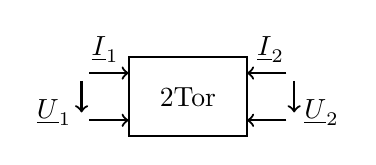
\begin{tikzpicture}[thick, ->]
  \draw (0,0.2) -- (0.5,0.2);
  \draw (0,0.8) -- (0.5,0.8) node[above left] {$\underline{I}_1$};
  \draw (-0.1,0.7) -- (-0.1,0.3) node[left] {$\underline{U}_1$};
  \draw (2.5,0.8) -- (2,0.8) node[above right] {$\underline{I}_2$};
  \draw (2.5,0.2) -- (2,0.2);
  \draw (2.6,0.7) -- (2.6,0.3) node[right] {$\underline{U}_2$};
  \draw (0.5,0) rectangle	(2,1);
  \node at (1.25,0.5) {2Tor};
\end{tikzpicture}\\
\textbf{Bsp/Aufgabe:} Man berechne $[\underline{A}]$ aus $[\underline{Z}]$\\

\begin{align}
	\underline{U}_1&=\underline{Z}_{11}\underline{I}_1+\underline{Z}_{12}\underline{I}_2\nonumber\\
	\underline{U}_2&=\underline{Z}_{21}\underline{I}_1+\underline{Z}_{22}\underline{I}_2\nonumber\\
	\nonumber\\
	\underline{U}_1&=\underline{A}_{11}\underline{U}_2+\underline{A}_{12}(\underline{-I}_2)\nonumber\\
	\underline{U}_1&=\underline{A}_{21}\underline{U}_2+\underline{A}_{22}(\underline{-I}_2)\nonumber\\
	\underline{I}_1&=\frac{1}{\underline{Z}_{21}}\left(\underline{U}_2-\underline{Z}_{22}\underline{I}_2\right)=\frac{1}{\underline{Z{21}}}\underline{U}_2+\frac{\underline{Z}_{22}}{\underline{Z}_{11}}\left(-\underline{I}_2\right)\nonumber\\
	\underline{U}_1&=\frac{\underline{Z}_{11}}{\underline{Z}_{21}}\underline{U}_2+\underline{Z}_{11}\frac{\underline{Z}_{12}}{\underline{Z}_{21}}\left(-\underline{I}_2\right)-\underline{Z}_{12}\left(-\underline{I}_2\right)\nonumber\\
	\underline{U}_1&=\frac{\underline{Z}_{11}}{\underline{Z}_{21}}\underline{U}_2+\underbrace{\left(\underline{Z}_{11}\frac{\underline{Z}_{22}}{\underline{Z}_{21}}-\underline{Z}_{12}\right)}_{\frac{\underline{Z}_{11}\underline{Z}_{22}-\underline{Z}_{12}\underline{Z}_{21}}{\underline{Z}_{21}}=\frac{det[Z]}{\underline{Z}_{21}}}\cdot\left(-\underline{I}_2\right)\nonumber\\
	[\underline{A}]&=\frac{1}{\underline{Z}_{21}}
	\begin{bmatrix}
		\underline{Z}_{11} & det[\underline{Z}]\\
		1 & \underline{Z}_{22}
	\end{bmatrix}\nonumber
\end{align}
\subsection{Parameter-Bestimmung}
\textbf{Bsp} Bild 2\\
\textbf{Ges:} $\underline{Z}$-Matrix\\
%TODO Z-Matrix formel
\begin{align}
	\underline{U}_1=\underline{Z}_{11}\underline{I}_1+\underline{Z}_{12}\underline{I}_2\nonumber\\
	\underline{U}_2=\underline{Z}_{21}\underline{I}_1+\underline{Z}_{22}\underline{I}_2\nonumber
	\end{align}\\
Zuerst allgemein als T-Glied\\
Bild 3\\
$\underline{Z}_{11}=?$
Falls $I_2=0$ (Ausg. offen)\\
\begin{align}
	\left. \underline{U}_1=\underline{Z}_{11}\underline{I}_1
	\right|_{\underline{I}_2=0}  \Rightarrow \underline{Z}_{11}=\frac{\underline{U}_1}{\underline{I}_1}=\underline{Z}_1+\underline{Z}_2\nonumber\\
	=\text{(primäre) Leerlaufimpedanz }\underline{Z}_{1l}\nonumber
\end{align}
$\underline{Z}_{12}=?$\\
\begin{align}
	\underline{U}_1&=\underline{Z}_{11}\underline{I}_1+\underline{Z}_{12}\underline{I}_2\nonumber\\
	\text{Falls } I_1&=0 \text{ Eingang offen}:\nonumber\\
	\underline{Z}_{12}&=\left.\frac{\underline{U}_1}{\underline{I}_2s}\right|_{\underline{I}_1=0}\nonumber
\end{align}
Bild 4\\
\begin{align}
	\underline{U}_1=\underline{Z}_2\underline{I}_2 \Rightarrow
	\frac{\underline{U}_1}{\underline{I}_2}=\underline{Z}_3=\underline{Z}_{12}\nonumber
\end{align}
$\underline{Z}_{22}=?$\\
\begin{align}
	\underline{U}_2&=\underline{Z}_{21}\underline{I}_1+\underline{Z}_{22}\underline{I}_2\nonumber\\
	\underline{Z}_{22}&=\left.\frac{\underline{U}_2}{\underline{I}_2}\right|_{I_1=0}=\underline{Z}_2+\underline{Z}_3\nonumber
\end{align}
$\underline{Z}_{21}=?$\\
\begin{align}
	\underline{Z}_{21}&=\left.\frac{\underline{U}_2}{\underline{I}_1}\right|_{I_2=0}=\underline{Z}_3\nonumber\\
	[\underline{Z}]&=
	\begin{bmatrix}
		\underline{Z}_1+\underline{Z}_3 & \underline{Z}_3\\
		\underline{Z}_3 & \underline{Z}_2+\underline{Z}_3
	\end{bmatrix}\nonumber\\
	[\underline{Z}]&=
	\begin{bmatrix}
		R+j\omega L & R\\
		R & R+\frac{1}{j\omega C}
	\end{bmatrix}\nonumber
\end{align}
Bild5\\
\begin{align}
	\underline{I}_1=\underline{Y}_11\underline{U}_1+\underline{Y}_12\underline{U}_2\nonumber\\
	\underline{I}_2=\underline{Y}_21\underline{U}_1+\underline{Y}_22\underline{U}_2\nonumber
\end{align}
$\underline{Y}_{11}=?$\\
\begin{align}	
	\underline{Y}_{11}&=\left.\frac{\underline{I}_1}{\underline{U}_1}\right|_{U_2=0}\nonumber\\
	U_2&=0: \text{ Kurzschluss am Ausgang}\nonumber\\
	\frac{\underline{I}_1}{\underline{U}_1}&=\underline{Y}_1+\underline{Y}_3=\underline{Y}_{11}\nonumber\\
	\underline{Y}_{11}&=\left.\frac{\underline{I}_1}{\underline{U}_2}\right|_{U_1=0}=-\underline{Y}_3\nonumber
\end{align}
Bild 6\\
Analog dazu:\\
\begin{align}
	\underline{Y}_{22}&=\underline{Y}_2+\underline{Y}_3\nonumber\\
	\underline{Y}_{21}&=\underline{Y}_3\nonumber
\end{align}
Daraus folgt:
\begin{align}
	[\underline{Y}]=
	\begin{bmatrix}
		\underline{Y}_1+\underline{Y}_3 & -\underline{Y}_3\\
		-\underline{Y}_3 & \underline{Y}_2+\underline{Y}_3
	\end{bmatrix}\nonumber
\end{align}
\textbf{Bsp}
Bild 7\\
\textbf{Ges:} $[\underline{A}=?]$\\
\begin{align}
	\underline{U}_1=\underline{A}_{11}\underline{U}_2+\underline{A}_{12}\left(-\underline{I}_2\right)\nonumber\\
	\underline{I}_1=\underline{A}_{21}\underline{U}_2+\underline{A}_{22}\left(-\underline{I}_2\right)\nonumber
\end{align}
$\underline{A}_{11}=?$\\
\begin{align}
	\underline{A}_{11}&=\left.\frac{\underline{U}_1}{\underline{U}_2}\right|_{\underline{I}_2=0}
	\rightarrow\text{ Quelle } \underline{U}_1 \text{anschliessen.}\nonumber\\
	\left.\frac{\underline{U}_2}{\underline{U}_1}\right|_{\underline{I}_2=0}&=\frac{\frac{1}{j\omega
	C}}{R+\frac{1}{j\omega C}}=\frac{1}{1+j\omega RC}\nonumber\\
	\rightarrow \underline{A}_{11}&=1+j\omega RC\nonumber
\end{align}
$\underline{A}_{12}=?$\\
\begin{align}
	\left.\underline{A}_{12}=\right|_{\underline{U}_2=0}\frac{\underline{U}_1}{-\underline{{I}_2}}\nonumber
\end{align}
Bild 8\\
$\underline{A}_{21}=?$\\
\begin{align}
	\underline{A}_{21}\left.=\right|_{\underline{I}_2=0}\frac{\underline{I}_1}{\underline{U}_2}\nonumber
\end{align}
Bild 9
\begin{align}
	\underline{U}_2&=\frac{\underline{I}_1}{j\omega C}\nonumber\\
	\frac{\underline{I}_1}{\underline{U}_2}&=j\omega C =
	\underline{A}_{21}\nonumber
\end{align}
$\underline{A}_{22}=?$\\
\begin{align}
	\underline{A}_{22}&=\left.\frac{\underline{I}_1}{-\underline{I}_2}\right|_{\underline{U}_2=0}=1\nonumber\\
	[A]&=
	\begin{bmatrix}
		1+j\omega RC & R\\
		j\omega C & 1
	\end{bmatrix}\nonumber
\end{align}
Beispiel Seite 55\\
\subsection{Leerlauf und Kurzschlussimpedanzen}
\textbf{Def}Bild 10\\
$\underline{Z}_{1l}=$ Primäre Leerlaufimpedanz\\
$\underline{Z}_{1k}=$ Primäre Kurzschlussimpedanz\\
$\underline{Z}_{2l}=$ Sekundäre Leerlaufimpedanz\\
$\underline{Z}_{2k}=$ Sekundäre Kurzschlussimpedanz\\
\subsubsection{Zusammenhang mit Zweitorparametern}
\begin{align}
	\underline{Z}_{1l}:
	\underline{U}_1&=\underline{Z}_11\underline{I}_1+\underline{Z}_{12}\underline{I}_2\nonumber\\
	\underline{Z}_{1l}&=\frac{\underline{U_1}}{\underline{I}_1}=\underline{Z}_{11}\nonumber\\
	\underline{Z}_{1k}:
	\underline{I}_1&=\underline{Y}_{11}\underline{U}_1+\underline{Y}_{12}\underline{U}_2\nonumber\\
	\underline{Z}_{1k}&=\frac{\underline{U}_1}{\underline{I}_1}=\frac{1}{\underline{Y}_{11}},
	\underline{Y}_{1k}=\underline{Y}_{11}\nonumber
\end{align}
\subsection{Leerlauf und Kurzschluss-Übertragungsgrössen}
\textbf{Bsp} (Leerlauf-)Spannungsübersetzung vorwärts\\
Vorwärts bedeutet speisung am Eingang\\
Bild 11\\
\begin{align}
	\underline{V}_{U21}&=\left.\frac{\underline{U}_2}{\underline{U}_1}\right|_{\underline{I}_2=0}=?\nonumber\\
	\underline{U}_1&=\underline{A}_{11}\underline{U}_{2}+\underline{A}_{12}\left(-\underline{I}_2\right)\nonumber\\
	%Nach 2. frac strich runter \underline{I}_2=0
	\frac{\underline{U}_2}{\underline{U}_1}&=\left.\frac{1}{\underline{A}_11}\right|_{\underline{I}_2=0}\nonumber
\end{align}
(Kurzschluss-)Übertragungsadmittanz vorwärts
$\frac{\underline{I}_2}{\underline{U}_1}$\\
Bild 12\\